\chapter{Fundamentos Geofísicos}

\section{Campo potencial gravitatorio}

Según la Ley de Gravitación Universal de Newton, una masa puntual $m_p$ situada
en la posición $\mathbf{p}$ siente una fuerza gravitatoria $\mathbf{F}$ debido
a la presencia de otra masa $m$ situada en la posición $\mathbf{q}$. Esta
fuerza puede expresarse como:

\begin{equation}
    \mathbf{F} = - G \frac{m_p m}{r^2} \mathbf{\hat{r}},
\end{equation}

\noindent donde $G = 6.67430 \times 10^{-11} \text{m}^3 \text{kg}^{-1}
\text{s}^{-2}$ es la constante de gravitación universal,
$\mathbf{r} = \mathbf{p} - \mathbf{q}$ es el vector que une $\mathbf{q}$ con
$\mathbf{p}$, y $\mathbf{\hat{r}}$ es el versor asociado a $\mathbf{r}$
(Fig.~\ref{fig:potencial-gravitatorio}a).
Aplicando la segunda Ley de Newton, se deduce que la masa $m_p$ siente una
aceleración gravitatoria $\mathbf{g}$:

\begin{equation}
    \mathbf{g} = - \frac{G m}{r^2} \mathbf{\hat{r}}.
    \label{eq:aceleracion-newton}
\end{equation}

Si consideramos que la partícula $m_p$ es una \emph{partícula de prueba},
podemos reescribir la ecuación \ref{eq:aceleracion-newton}, pero ahora
resignificándola como la aceleración gravitatoria que sentiría cualquier
partícula localizada en un punto $\mathbf{p}$ debido a la presencia de la
partícula $m$:

\begin{equation}
    \mathbf{g}(\mathbf{p}) = - \frac{G m}{r^2} \mathbf{\hat{r}}.
\end{equation}

Se puede demostrar que la atracción gravitatoria $\mathbf{g}$ define un campo
irrotacional, es decir:

\begin{equation}
    \nabla \times \mathbf{g} = 0.
\end{equation}

\noindent Por ende es posible definir un potencial escalar $V$ al que
denominaremos \emph{potencial gravitatorio}:

\begin{equation}
    \mathbf{g}(\mathbf{p}) = + \nabla V(\mathbf{p}),
    \label{eq:potencial-gravitatorio-definicion}
\end{equation}

\noindent donde

\begin{equation}
    V(\mathbf{p}) = G \frac{m}{r}.
\end{equation}

\noindent Vale la pena notar que en la ecuación
\ref{eq:potencial-gravitatorio-definicion} se ha aplicado la convención de
signo positivo para definir el potencial $V$, mayormente utilizada en la
literatura sobre Geofísica y Geodesia
\citep{heiskanen1967,blakely1995,hinze2009}.

\begin{figure}
    \centering
    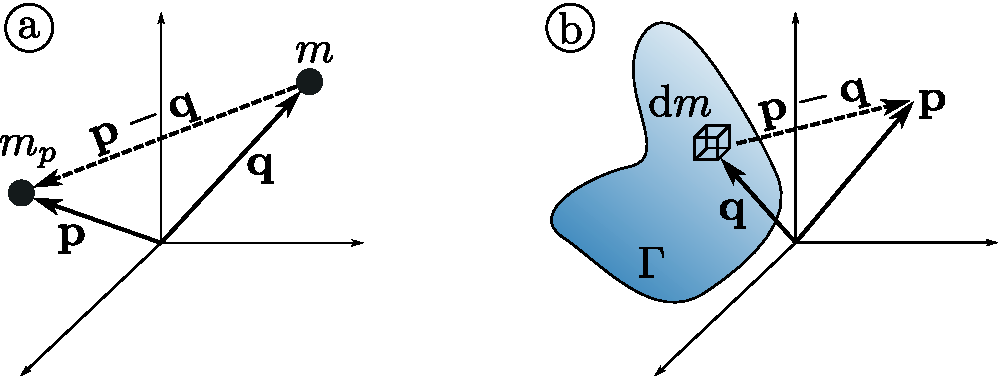
\includegraphics[width=\linewidth]{figs/gravity-potentials.pdf}
    \caption{
        (a)~Masas puntuales $m_p$ y $m$ localizadas en $\mathbf{p}$
        y $\mathbf{q}$, respectivamente. El vector $\mathbf{r}$ se define como
        $\mathbf{p} - \mathbf{q}$.
        (b)~Distribución de masa $\Gamma$, diferencial de masa $\text{d}m$
        ubicado en el punto $\mathbf{q}$.
    }
    \label{fig:potencial-gravitatorio}
\end{figure}


\subsection{Potencial gravitatorio producido por una distribución de masa}

Partiendo de que un diferencial de masa $\text{d}m$ ubicado en $\mathbf{q}$
genera un potencial gravitatorio $\text{d}V$ en cualquier punto $\mathbf{p}$
(Fig.~\ref{fig:potencial-gravitatorio}b):

\begin{equation}
    \text{d}V(\mathbf{p}) = \frac{G}{|\mathbf{p} - \mathbf{q}|} \text{d}m,
\end{equation}

\noindent el potencial gravitatorio generado por una distribución de masa
$\Gamma$ puede calcularse integrando los diferenciales de masa que lo componen:

\begin{equation}
    V(\mathbf{p}) =
        G \int\limits_\Gamma \frac{\text{d}m}{|\mathbf{p} - \mathbf{q}|} .
\end{equation}

Si reescribimos los diferenciales de masa como

\begin{equation}
    \text{d}m = \rho(\mathbf{q}) \text{d}v,
\end{equation}

\noindent donde $\rho(\mathbf{q})$ es la densidad de masa de la distribución
$\Gamma$ en el punto $\mathbf{q}$ y $\text{d}v$ es el diferencial de volumen,
el potencial se puede expresar como:

\begin{equation}
    V(\mathbf{p}) =
        G \int\limits_\Gamma
        \frac{\rho(\mathbf{q})}{|\mathbf{p} - \mathbf{q}|} \text{d}v.
    \label{eq:potencial-gravitatorio-integral}
\end{equation}


\subsection{Gradiente del potencial gravitatorio}

Según la definición del potencial gravitatorio expuesta en la
ecuación~\ref{eq:potencial-gravitatorio-definicion}, es posible calcular la
aceleración de la gravedad producida por una distribución de masa arbitraria
en cualquier punto $\mathbf{p}$ como el gradiente del potencial
$V(\mathbf{p})$.
Si definimos un sistema de ejes Cartesianos en el cual el punto $\mathbf{p}
= (x, y, z)$, las componentes de la aceleración en cada una de las direcciones
del sistema quedan expresadas
como:

\begin{equation}
    g_i(\mathbf{p}) = \frac{\partial V(\mathbf{p})}{\partial i}, \,\,
        \forall i \in \{x, y, z\}.
    \label{eq:componentes-aceleracion-gravitatoria}
\end{equation}

El vector
$\mathbf{g}(\mathbf{p}) = (g_x(\mathbf{p}), g_y(\mathbf{p}), g_z(\mathbf{p}))$
representa la aceleración gravitatoria en el punto
$\mathbf{p}$ generada por la distribución de masa $\Gamma$, aunque es común
referirse al mismo como el \emph{gradiente gravitatorio}.
Reemplazando la ecuación~\ref{eq:potencial-gravitatorio-integral}
en~\ref{eq:componentes-aceleracion-gravitatoria}, las componentes del gradiente
gravitatorio pueden expresarse como:

\begin{align}
    g_x(\mathbf{p}) =&
        - G \int\limits_\Gamma \rho(\mathbf{q})
        \frac{(x - x')}{|\mathbf{p} - \mathbf{q}|^2} \text{d}v, \\
    g_y(\mathbf{p}) =&
        - G \int\limits_\Gamma \rho(\mathbf{q})
        \frac{(y - y')}{|\mathbf{p} - \mathbf{q}|^2} \text{d}v, \\
    g_z(\mathbf{p}) =&
        - G \int\limits_\Gamma \rho(\mathbf{q})
        \frac{(z - z')}{|\mathbf{p} - \mathbf{q}|^2} \text{d}v,
\end{align}

\noindent donde $\mathbf{q} = (x', y', z')$.

Las segundas derivadas del potencial gravitatorio definen el \emph{tensor del
gradiente gravitatorio}, y sus componentes pueden expresarse como:

\begin{equation}
    g_{ij}(\mathbf{p}) =
        \frac{\partial^2 V(\mathbf{p})}{\partial i \partial j}, \,\,
        \forall i \in \{x, y, z\}, \,\,
        \forall j \in \{x, y, z\}.
\end{equation}

Reemplazando la ecuación \ref{eq:potencial-gravitatorio-integral}, podemos
expresar las componentes diagonales del tensor de la siguiente manera
\citep{grombein2013}:

\begin{align}
    g_{xx}(\mathbf{p}) =&
        G \int\limits_\Gamma \rho(\mathbf{q})
        \left[
        \frac{3(x - x')^2}{|\mathbf{p} - \mathbf{q}|^5}
        - \frac{1}{|\mathbf{p} - \mathbf{q}|^3}
        \right]
        \text{d}v, \\
    g_{yy}(\mathbf{p}) =&
        G \int\limits_\Gamma \rho(\mathbf{q})
        \left[
        \frac{3(y - y')^2}{|\mathbf{p} - \mathbf{q}|^5}
        - \frac{1}{|\mathbf{p} - \mathbf{q}|^3}
        \right]
        \text{d}v, \\
    g_{zz}(\mathbf{p}) =&
        G \int\limits_\Gamma \rho(\mathbf{q})
        \left[
        \frac{3(z - z')^2}{|\mathbf{p} - \mathbf{q}|^5}
        - \frac{1}{|\mathbf{p} - \mathbf{q}|^3}
        \right]
        \text{d}v,
    \label{eq:componentes-diagonales-tensor}
\end{align}

\noindent mientras que las componentes no diagonales pueden expresarse como:

\begin{align}
    g_{xy}(\mathbf{p}) =
    g_{yx}(\mathbf{p}) =&
        G \int\limits_\Gamma \rho(\mathbf{q})
        \frac{3(x - x')(y - y')}{|\mathbf{p} - \mathbf{q}|^5}
        \text{d}v, \\
    g_{xz}(\mathbf{p}) =
    g_{zx}(\mathbf{p}) =&
        G \int\limits_\Gamma \rho(\mathbf{q})
        \frac{3(x - x')(z - z')}{|\mathbf{p} - \mathbf{q}|^5}
        \text{d}v, \\
    g_{yz}(\mathbf{p}) =
    g_{zy}(\mathbf{p}) =&
        G \int\limits_\Gamma \rho(\mathbf{q})
        \frac{3(y - y')(z - z')}{|\mathbf{p} - \mathbf{q}|^5}
        \text{d}v.
\end{align}

A partir de las ecuaciones \ref{eq:componentes-diagonales-tensor} podemos
calcular el Laplaciano del potencial gravitatorio:

\begin{equation}
    \Delta V(\mathbf{p}) = \nabla^2 V(\mathbf{p}) =
        \frac{\partial^2 V}{\partial x^2}
        + \frac{\partial^2 V}{\partial y^2}
        + \frac{\partial^2 V}{\partial z^2},
\end{equation}

\noindent Dado que las tres expresiones se cancelan mutuamente
\citep{blakely1995}, podemos concluir que cualquier potencial gravitatorio es
un \emph{campo harmónico}

\begin{equation}
    \Delta V(\mathbf{p}) = 0
\end{equation}

\noindent para cualquier punto de observación $\mathbf{p}$.

% =============================================================================

\section{Modelado directo}

El cálculo de los efectos gravitatorios de un determinado cuerpo sobre uno
o más puntos de observación se suele denominar modelado directo (\emph{forward
modelling} en inglés).
Aunque las expresiones del potencial gravitatorio y las componentes de su
gradiente en las
ecuaciones~\ref{eq:potencial-gravitatorio-integral} y
\ref{eq:componentes-aceleracion-gravitatoria} aparentan ser sencillas, el
cómputo de estas magnitudes para una geometría dada no resulta un problema
trivial.
Solo existen soluciones analíticas a dichas expresiones para determinadas
geometrías sencillas o que guardan algún tipo de simetría.

En el desarrollo de esta Tesis nos resultan de principal interés trabajar con
tres tipos de geometrías: masas puntuales, prismas rectangulares y prismas
esféricos o \emph{tesseroides}.

\subsection{Masas puntuales}

\subsection{Prismas rectangulares}

\subsection{Tesseroides}

% =============================================================================

\section{Disturbio de gravedad}

\subsection{Elipsoide de referencia}

\section{Fuentes equivalentes}
